\documentclass{article}
\usepackage[utf8]{inputenc}
\usepackage{amsmath, amsthm, amsfonts,amssymb}
\usepackage[spanish]{babel}
\usepackage{multicol}
\usepackage{listings}
\lstset{basicstyle=\footnotesize\ttfamily,breaklines=true}
\usepackage{alltt}
\usepackage{graphicx}
\usepackage{subfigure}
\usepackage{subfig}
\usepackage{float}
\usepackage{url}
\usepackage{enumerate}
\usepackage{color}
\usepackage{cancel}
\usepackage{wrapfig}\definecolor{shadecolor}{RGB}{250,250,250}
\usepackage{framed}
\usepackage{epstopdf}
\setlength\parindent{0pt}
\usepackage{listings}
\usepackage{color} %red, green, blue, yellow, cyan, magenta, black, white
% Operadores matemáticos y simbolos
\DeclareMathOperator{\dive}{div}
\DeclareMathOperator{\trace}{trace}
\DeclareMathOperator{\tr}{tr}
\DeclareMathOperator{\symm}{symm}
\DeclareMathOperator{\sk}{skew}
\DeclareMathOperator{\grad}{grad}
\DeclareMathOperator{\Grad}{Grad}
\DeclareMathOperator{\curl}{curl}
\DeclareMathOperator{\Curl}{Curl}
\def\R{\mbox{\(\mathbb{R}\)}}
\def\E{\mbox{\(\mathbb{E}\)}}
\def\P{\mbox{\(\mathbb{P}\)}}
\def\I{\mbox{\(\mathbb{I}\)}}
\def\L{\mbox{\(\mathbb{L}\)}}
\def\dx{\mbox{\(\,\mathrm{d}x\)}}
\usepackage{changepage}
\usepackage[showframe=false]{geometry}
\geometry{left=2.5cm, right=2.5cm, top=2cm, bottom=3cm}
\title{Tarea 2\\}
\author{Luis Felipe Silva De Vidts}
\begin{document}
\begin{figure}
\begin{minipage}{2.5cm}

\includegraphics[width=0.8\textwidth]{./figures/LogoUC-BN}
\end{minipage}
\begin{minipage}{14.5cm}
\vspace{4mm}
{\sc PONTIFICIA UNIVERSIDAD CAT\'OLICA DE CHILE}\\
Facultad de Matemáticas\\
Departamento de Estadísica\\
{\bf EYP1113 Probabilidades y Estadística}\\
\vspace{0mm}
\hrulefill
\end{minipage}
\end{figure}
\phantom{""}
\vspace{-5mm}
\normalsize
\begin{center}
\Huge Tarea 2\\
\normalsize Luis Felipe Silva De Vidts
\end{center}
\section*{Estadística descriptiva}
Tabla con todas las medidas descriptivas de todas las variables de la base entregada.
\begin{figure}[h!]
\begin{adjustwidth}{-2cm}{}
\begin{tabular}{|c|c|c|c|c|c|c|c|c|c|}
\hline
           & Min.&      1st Qu. &      Median  &       Mean &     3rd Qu. &        Max. &          SD   &   Skewness &  Kurtosis\\
\hline
año       & 2003 & 2006 & 2010 & 2009.7167 & 2013 & 2017  &  4.1785  &1.2258e-02 &-1.2148\\
\hline
mes      &     1  &   3 &    6 &    6.3988 &    9   & 12  &  3.4703  &4.2794e-02& -1.2441\\
\hline
tiempo  &   2003 & 2006.5833 & 2010.1666 & 2010.1666 & 2013.75 &2017.3333  & 4.1737 &-9.4398e-14 &-1.2208\\
\hline
tasa   &       3.2472 &    4.4473  &   4.7248 &    4.7626 &    5.0184  &   6.7493   & 0.7733 & 5.4080e-01 & 0.3163\\
\hline
desempleo    & 5.6902 &    6.5  &  7.3300 &    7.6920  &   8.7504  &  11.2180   & 1.4784  &6.3350e-01 &-0.7240\\
\hline
imacec      & 59.8227 &   76.7760   & 85.0768 &   87.0702  &  99.46  & 116.0323  & 13.8430 & 4.7584e-02 &-1.1324\\
\hline
bcu        &   1.118 &    2.1933   &  2.7366 &    2.6165  &   3.1341 &    4.2961   & 0.7743 &-1.8774e-01& -0.6912\\
\hline
pib       &21320.3553& 26182.3902& 28566.2587& 29815.6212 &34763.6470 &36602.6629 &4778.1374 &-1.0556e-01 &-1.2528\\
\hline
\end{tabular}
\end{adjustwidth}
\end{figure}
A continuacion todos los gráficos de cada una de las variables, histograma, boxplot y como ajustan a 6 distintas distribuciones de probabilidad.
\begin{figure}[h!]
\centering
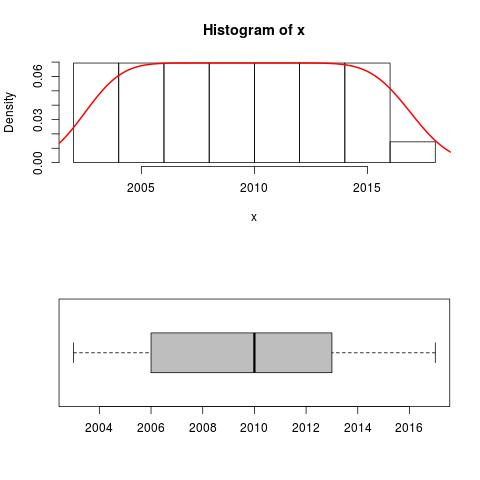
\includegraphics[scale=0.5]{./plots/histplot_a_o.png}
\caption{Histograma y Boxplot de año}
\end{figure}

\begin{figure}[h!]
\centering
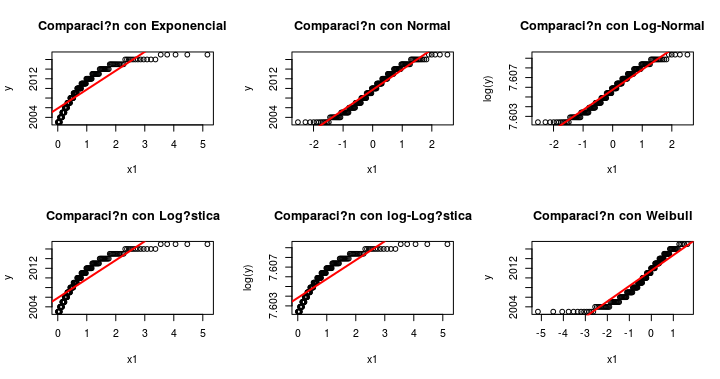
\includegraphics[scale=0.5]{./plots/cm_a_o.png}
\caption{Comparación con modelos de año}
\end{figure}

\begin{figure}[h!]
\centering
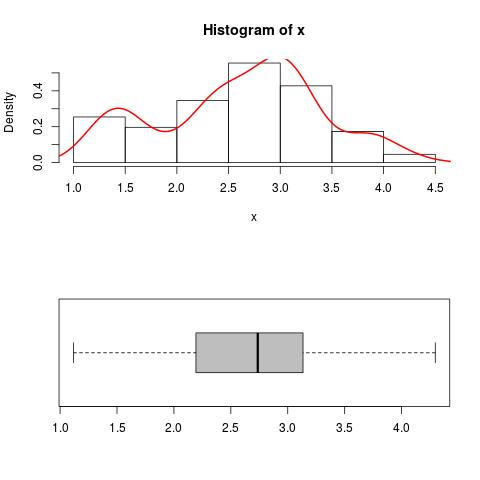
\includegraphics[scale=0.5]{./plots/histplot_bcu.png}
\caption{Histograma y Boxplot de bcu}
\end{figure}

\begin{figure}[h!]
\centering
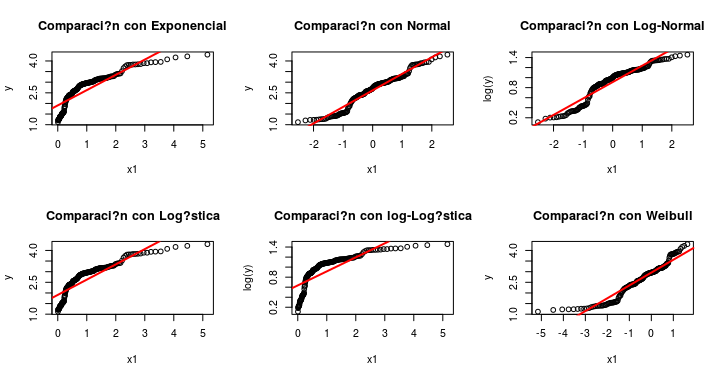
\includegraphics[scale=0.5]{./plots/cm_bcu.png}
\caption{Comparación con modelos de bcu}
\end{figure}
\pagebreak
\begin{figure}[h!]
\centering
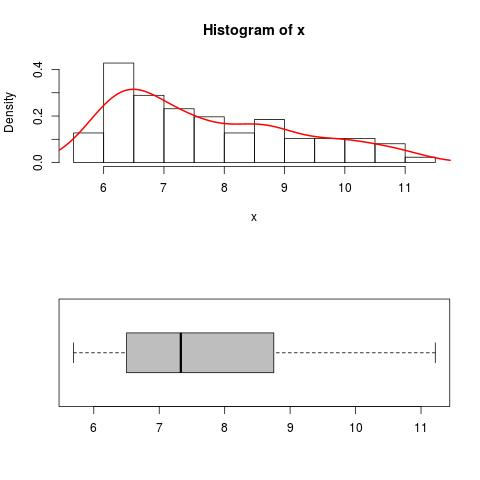
\includegraphics[scale=0.5]{./plots/histplot_desempleo.png}
\caption{Histograma y Boxplot de desempleo}
\end{figure}

\begin{figure}[h!]
\centering
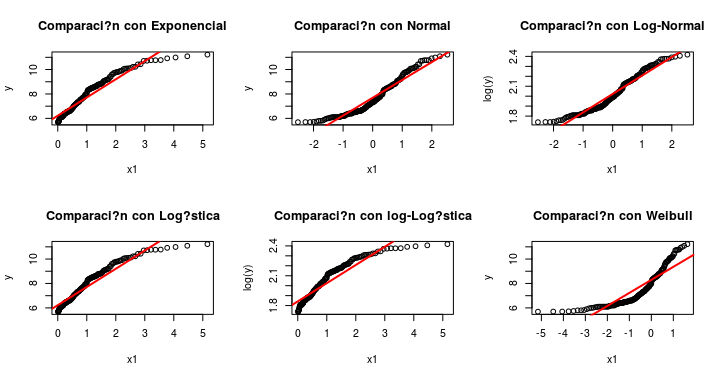
\includegraphics[scale=0.5]{./plots/cm_desempleo.png}
\caption{Comparación con modelos de desempleo}
\end{figure}
\pagebreak
\begin{figure}[h!]
\centering
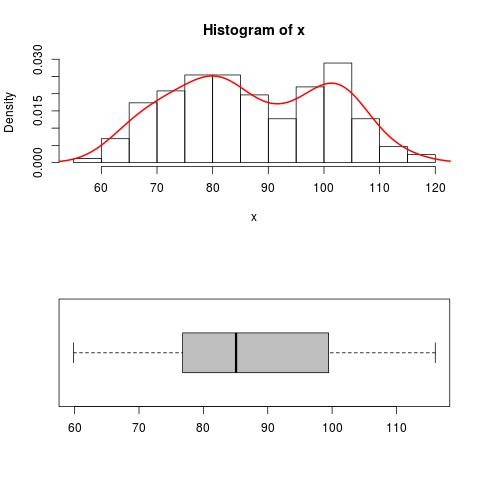
\includegraphics[scale=0.5]{./plots/histplot_imacec.png}
\caption{Histograma y Boxplot de imacec}
\end{figure}

\begin{figure}[h!]
\centering
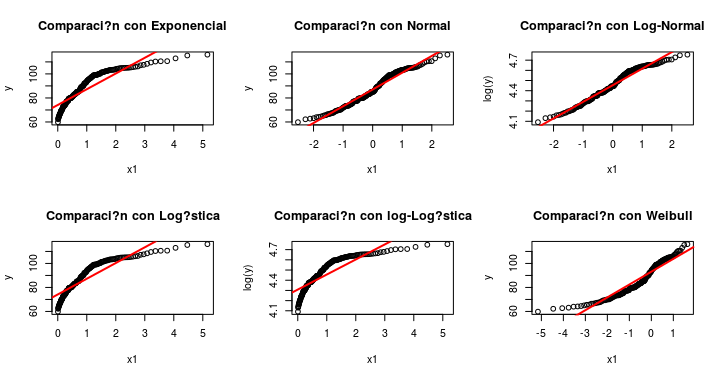
\includegraphics[scale=0.5]{./plots/cm_imacec.png}
\caption{Comparación con modelos de imacec}
\end{figure}
\pagebreak
\begin{figure}[h!]
\centering
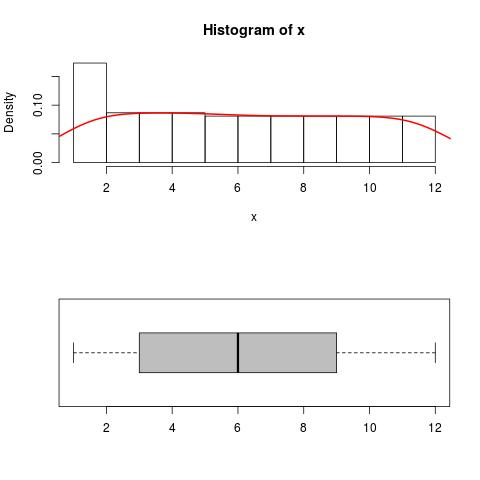
\includegraphics[scale=0.5]{./plots/histplot_mes.png}
\caption{Histograma y Boxplot de mes}
\end{figure}

\begin{figure}[h!]
\centering
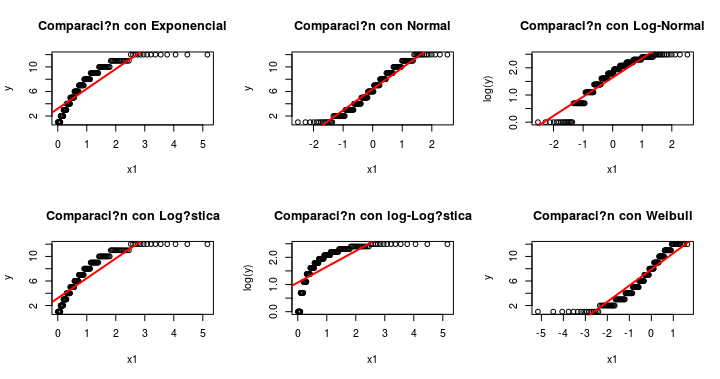
\includegraphics[scale=0.5]{./plots/cm_mes.png}
\caption{Comparación con modelos de mes}
\end{figure}
\pagebreak
\begin{figure}[h!]
\centering
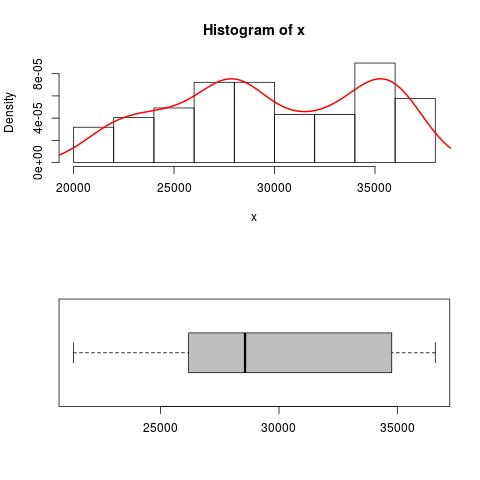
\includegraphics[scale=0.5]{./plots/histplot_pib.png}
\caption{Histograma y Boxplot de pib}
\end{figure}

\begin{figure}[h!]
\centering
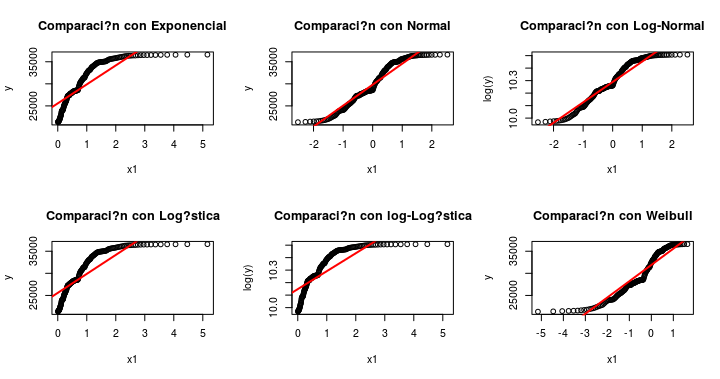
\includegraphics[scale=0.5]{./plots/cm_pib.png}
\caption{Comparación con modelos de pib}
\end{figure}
\pagebreak
\begin{figure}[h!]
\centering
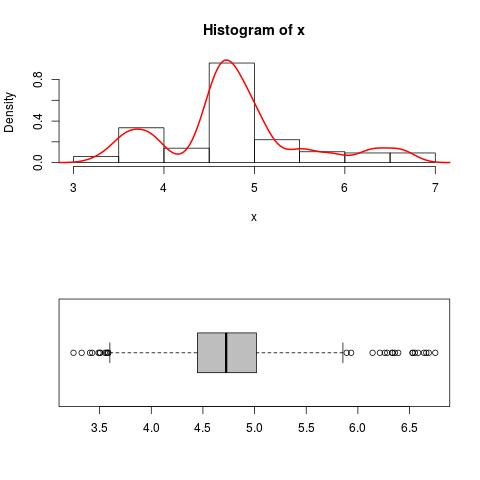
\includegraphics[scale=0.5]{./plots/histplot_tasa.png}
\caption{Histograma y Boxplot de tasa}
\end{figure}

\begin{figure}[h!]
\centering
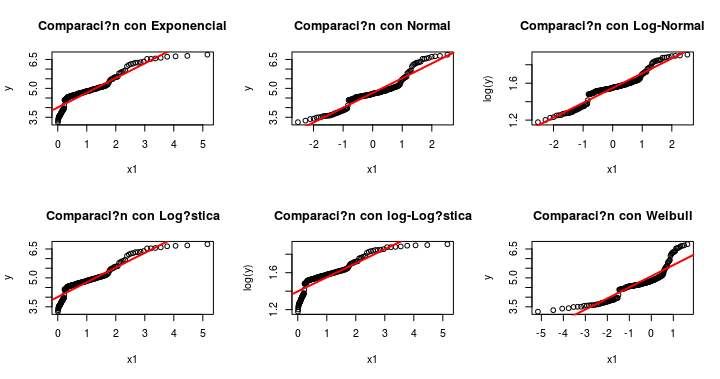
\includegraphics[scale=0.5]{./plots/cm_tasa.png}
\caption{Comparación con modelos de tasa}
\end{figure}

\begin{figure}[h!]
\centering
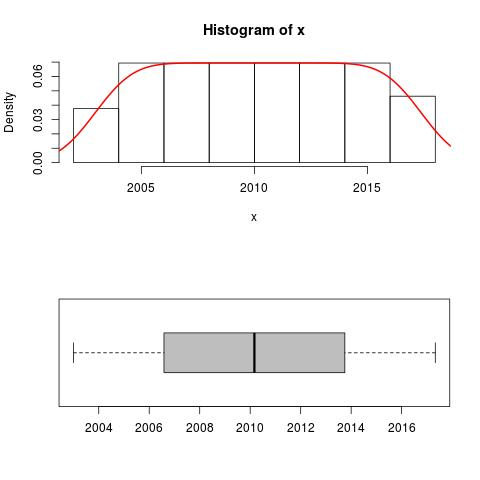
\includegraphics[scale=0.5]{./plots/histplot_tiempo.png}
\caption{Histograma y Boxplot de tiempo}
\end{figure}

\begin{figure}[h!]
\centering
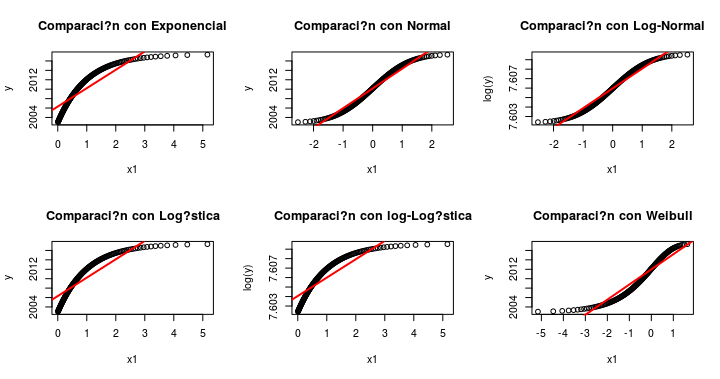
\includegraphics[scale=0.5]{./plots/cm_tiempo.png}
\caption{Comparación con modelos de tiempo}
\end{figure}
\pagebreak
\section*{IMACEC vs demás variables}
Al generar lo modelos lineales obtenemos que:

\begin{figure}[h!]
\begin{tabular}{|c|c|c|c|c|}
\hline
Imacec v/s & valor-p & $r^{2}$-ajustado& $R^{2}$& qf(0.95) vs F-Stadistic \\
\hline
tasa & $< 2.2e-16$ & 0.5711 & 0.5736&$3.896415<230.1$\\
\hline
bcu & $< 2.2e-16$ &  0.6934  & 0.6952& $3.896415<390$\\
\hline
desempleo & $< 2.2e-16$ & 0.6308  & 0.6329& $3.896415<294.8$\\
\hline
pib & $< 2.2e-16$ & 0.9299 &0.9303&$3.896415<2284$\\
\hline
\end{tabular}

\end{figure}
donde notamos que la variable que mejor describe al imacec de forma lineal\footnote{No alcance a aprender a usar bien el comando nls, por lo que no pude probar con un ajuste no lineal} es el PIB, tanto por test-f como por $r^{2}$ ajustado y  $R^{2}$.


\section*{Agregando el efecto MES}
\begin{figure}[h!]
\centering
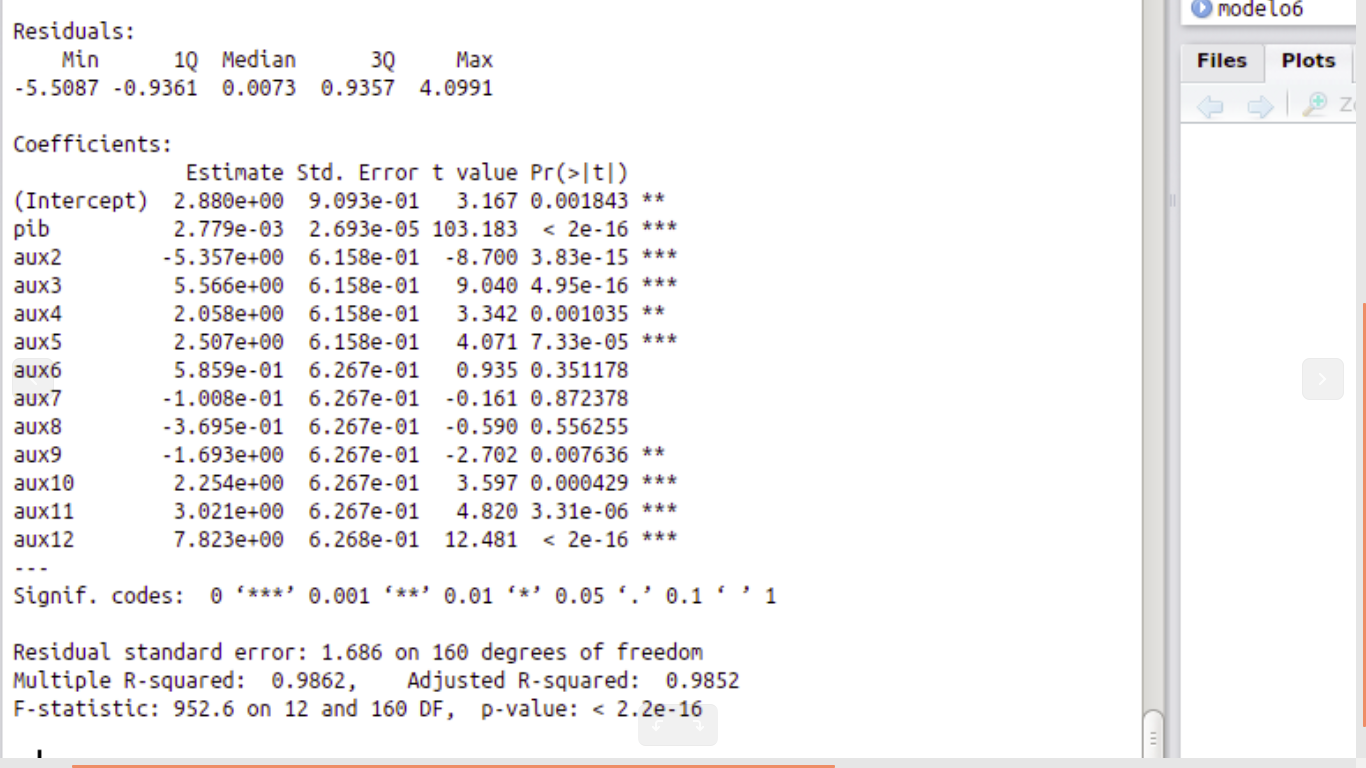
\includegraphics[scale=0.5]{./plots/salida_final_R.png}
\caption{Salida de R para el modelo considerando mes}
\end{figure}
En este caso notamos que mejoran los valores de todos los estadísticos, F-Stadistic, $r^{2}$-ajustado y $R^{2}$, además de que los primeros meses y los últimos del año explican mejor el imacec que los meses de mediania del año.
\section*{Aplicación Regresión Forward}
Al agregar variables al método anterior, solo hubo una pequeña disminución del $r^{2}$-ajustado, por lo que no agregue ninguna variable extra al modelo.
\section*{Tests de  Normalidad}
\end{document}
